\chapter{Elektromagnetische energie en de
poyntingvector}\label{ch:b2:poynting-vector}

Een batterij laat een lampje branden via twee koperdraden. Waar reist de
energie? Niet in het koper, zo blijkt: de elektronen daar driften met een
millimeter per seconde en dragen zo goed als niets. De energie stroomt door
de \emph{ruimte om de draden heen}, in het elektromagnetische veld, en komt
de gloeidraad van het lampje via zijn zijkant binnen. De zon levert op
precies dezelfde manier een kilowatt aan elke vierkante meter zonnig dak,
over honderdvijftig miljoen kilometer vacuüm. Dit hoofdstuk leidt uit de
\omterm{thm:b2:maxwell-equations:maxwell}{vergelijkingen van Maxwell} de balans van de elektromagnetische energie af
--- hoeveel er in een veld is opgeslagen, en de vector van Poynting, die
zegt waar zij heen gaat --- en past die toe op een draad, een condensator,
een spoel en een lichtbundel.

\section{De energiebalans van het veld}

\begin{theorem}[Stelling van Poynting]\label{thm:b2:poynting-vector:poynting}
\index{poyntingvector}\index{stelling van Poynting}\index{elektromagnetische energiedichtheid}
Definieer de \emph{\omterm{thm:b2:poynting-vector:poynting}{elektromagnetische energiedichtheid}} en de \emph{\omterm{thm:b2:poynting-vector:poynting}{poyntingvector}}
\[
u = \frac{\varepsilon_0E^2}2 + \frac{B^2}{2\mu_0} \quad (\unit{J/m^3}) , \qquad
\vect\Pi = \frac{\vect E\wedge\vect B}{\mu_0} \quad (\unit{W/m^2}) .
\]
De \omterm{thm:b2:maxwell-equations:maxwell}{vergelijkingen van Maxwell} houden dan in elk punt in dat
\[
\frac{\partial u}{\partial t} + \operatorname{div}\vect\Pi = -\vect j\cdot\vect E ,
\]
en, voor elk vast volume $V$ begrensd door $\Sigma$,
\[
\frac{\dd}{\dd t}\iiint_Vu\,\dd\tau = -\iint_\Sigma\vect\Pi\cdot\vect n\,\dd S - \iiint_V\vect j\cdot\vect E\,\dd\tau :
\]
de veldenergie binnen $V$ neemt af met wat er door de rand naar buiten
stroomt --- de flux van $\vect\Pi$ --- en met wat het veld aan de ladingen
geeft ($\vect j\cdot\vect E$, het vermogen van Joule in een geleider).
$\vect\Pi$ is de dichtheid van de energieflux: het vermogen dat een
eenheidsoppervlak loodrecht erop passeert.
\end{theorem}

\begin{proof}
Uit Maxwell--Ampère volgt
$\vect j = \operatorname{\vect{curl}}\vect B/\mu_0 - \varepsilon_0\partial_t
\vect E$,
zodat
$\vect j\cdot\vect E = \vect E\cdot\operatorname{\vect{curl}}\vect B/\mu_0 -
\partial_t(\varepsilon_0E^2/2)$.
De identiteit
$\operatorname{div}(\vect E\wedge\vect B) = \vect B
\cdot\operatorname{\vect{curl}}\vect E - \vect E\cdot\operatorname{\vect{curl}}\vect B$
(ga haar op de componenten na) en Maxwell--Faraday geven
$\vect E\cdot\operatorname{\vect{curl}}
\vect B = -\operatorname{div}(\vect E\wedge\vect B) - \vect B\cdot\partial_t\vect B = -\mu_0
\operatorname{div}\vect\Pi - \partial_t(B^2/2)$.
Samengenomen:
$\vect j\cdot\vect E = -\operatorname{div}
\vect\Pi - \partial_tu$.
Integreer over $V$ en pas de divergentiestelling toe.
\end{proof}

\begin{remark}[Wat vastligt en wat niet]\label{rem:b2:poynting-vector:interpretation}
De stelling legt alleen de flux van $\vect\Pi$ door gesloten oppervlakken en
de totale $u$ vast; elk divergentievrij veld bij $\vect\Pi$ optellen zou
niets waarneembaars veranderen. De bovenstaande keuze is de eenvoudigste,
zij stemt overeen met de impuls die het licht draagt (hieronder), en zij
wordt overal gebruikt. De dichtheden $\varepsilon_0E^2/2$ en $B^2/2\mu_0$
zijn de energieën van de condensator en de spoel van het volume van jaar 1,
nu aan elk punt van de ruimte toegekend: een veld van \qty{1}{MV/m} (de
doorslaggrens van lucht) slaat \qty{4.4}{J/m^3} op, een veld van \qty{1}{T}
slaat \qty{0.4}{MJ/m^3} op --- honderdduizend keer meer, en daarom haalt
energieopslag in magneten, en niet in condensatoren, de megajoule.
\end{remark}

\section{Waar de energie stroomt: drie schakelingen}

\begin{example}[De weerstandsdraad]\label{ex:b2:poynting-vector:wire}
Een cilindrische draad met straal $a$ voert de constante stroom $I$ onder
het veld $E = j/\gamma$ langs zijn as; vlak erbuiten is $B = \mu_0I/2\pi a$
(azimutaal). Aan het oppervlak wijst $\vect\Pi = \vect E\wedge\vect B/\mu_0$
\emph{radiaal naar binnen}, met grootte $EI/2\pi a$; haar flux door het
zijoppervlak van een lengte $L$ is
$EI/2\pi a\times2\pi aL = (EL)I = UI =
RI^2$: de warmte van Joule komt de
draad via zijn zijkant binnen, geleverd door het omringende veld, en wordt
niet door de elektronen door de draad meegevoerd. Binnenin is
$\Pi(r) = (E/\mu_0)(\mu_0Ir/2\pi a^2) = EIr/2\pi a^2$: de instroom neemt
naar de as toe af naarmate de energie laag voor laag wordt afgezet.
\end{example}

\begin{example}[De condensator en de solenoïde]\label{ex:b2:poynting-vector:capsol}
Een condensator met ronde platen die wordt geladen: $\vect E$ axiaal,
$\vect B =
\mu_0\varepsilon_0(r/2)\dot E\,\vect e_\theta$
(\cref{ch:b2:maxwell-equations}), zodat
$\vect\Pi = -\varepsilon_0(r/2)E\dot E\,\vect e_r$, naar binnen gericht;
door de cilinder met straal $R$ en hoogte $d$ is haar flux
$\varepsilon_0\pi R^2d\,E\dot E = \dd(\tfrac12
\varepsilon_0E^2\,\pi R^2d)/\dd t$:
de elektrische energie komt vanaf de rand binnen. Een solenoïde waarvan de
stroom groeit: $\vect B$ axiaal, het geïnduceerde
$\vect E = -(r/2)
\dot B\,\vect e_\theta$,
$\vect\Pi = -(rB\dot B/2\mu_0)\vect e_r$, opnieuw naar binnen, met flux
$\dd(B^2/2\mu_0\times\text{volume})/\dd t$. In elk geval bereikt de energie
het toestel door het veld erbuiten; de draden geleiden alleen het veld.
\end{example}

\begin{omfigure}
\begin{tikzpicture}[font=\small, x=1cm, y=1cm, >=Stealth]
  \begin{scope}
    \draw[thick, fill=omExo!20] (-2.4,-0.5) rectangle (2.4,0.5);
    \draw[omDef, thick, ->] (-1.6,0) -- (-0.6,0) node[above, font=\footnotesize] {$\vect E$};
    \draw[omDef, thick, ->] (0.6,0) -- (1.6,0);
    \node[omProp, font=\footnotesize] at (0,0.8) {$\odot\ \vect B$}; \node[omProp, font=\footnotesize] at (0,-0.8) {$\otimes\ \vect B$};
    \foreach \x in {-1.8,-0.9,0,0.9,1.8} {\draw[omThm, thick, ->] (\x,1.4) -- (\x,0.6); \draw[omThm, thick, ->] (\x,-1.4) -- (\x,-0.6);}
    \node[omThm, font=\footnotesize] at (2.5,1.1) {$\vect\Pi$};
    \node[font=\footnotesize] at (0,-1.85) {draad: $\vect\Pi$ naar binnen, flux $= RI^2$};
  \end{scope}
  \begin{scope}[xshift=7.2cm]
    \draw[thick, fill=omExo!40] (-0.9,-1.3) rectangle (-0.75,1.3); \draw[thick, fill=omExo!40] (0.75,-1.3) rectangle (0.9,1.3);
    \foreach \y in {-0.9,-0.45,0,0.45,0.9} \draw[omDef, ->] (-0.7,\y) -- (0.7,\y);
    \node[omDef, font=\footnotesize] at (0,1.55) {$\vect E$ groeit};
    \foreach \y in {-1.0,-0.5,0,0.5,1.0} {\draw[omThm, thick, ->] (1.9,\y) -- (1.05,\y); \draw[omThm, thick, ->] (-1.9,\y) -- (-1.05,\y);}
    \node[omThm, font=\footnotesize] at (2.2,1.3) {$\vect\Pi$};
    \node[font=\footnotesize] at (0,-1.85) {condensator: de energie komt van de rand binnen};
  \end{scope}
\end{tikzpicture}

{\small Links: een stroomvoerende draad --- de \omterm{thm:b2:poynting-vector:poynting}{poyntingvector}, opgebouwd uit
de axiale $\vect E$ en de azimutale $\vect B$, wijst rondom het hele
oppervlak de draad in; de warmte van Joule komt via de zijkant binnen.
Rechts: een condensator die wordt geladen --- de energie stroomt radiaal
door de spleet naar binnen, niet door de platen.}
\end{omfigure}

\begin{remark}[Energie in een statisch gekruist veld]\label{rem:b2:poynting-vector:static}
Een geladen condensator in het veld van een permanente magneet heeft overal
tussen zijn platen $\vect\Pi = \vect E\wedge\vect B/\mu_0 \ne \vect 0$,
hoewel er niets verandert en niets warm wordt. Er is geen tegenspraak:
$\vect\Pi$ heeft daar \omterm{def:b2:maxwell-equations:operators}{divergentie} nul, haar lijnen sluiten zich, en haar
flux door elk gesloten oppervlak verdwijnt --- de stelling zegt niets over
een circulerende stroming die niets aflevert. Alleen fluxen door gesloten
oppervlakken zijn fysisch.
\end{remark}

\begin{omfigure}
\begin{tikzpicture}[font=\small, x=1cm, y=1cm, >=Stealth]
  \begin{scope}
    \draw[thick, fill=omExo!30] (0,0) circle (1.6); \draw[thick, fill=omDef!10] (0,0) circle (1.35); \draw[thick, fill=omExo!60] (0,0) circle (0.35);
    \foreach \a in {0,45,...,315} \draw[omDef, ->] ({0.4*cos(\a)},{0.4*sin(\a)}) -- ({1.1*cos(\a)},{1.1*sin(\a)});
    \draw[omProp, thick, ->] (0.85,0) arc[start angle=0, end angle=300, radius=0.85];
    \node[omDef, font=\footnotesize] at (1.0,1.35) {$\vect E$}; \node[omProp, font=\footnotesize] at (-0.55,-1.05) {$\vect B$};
    \node[font=\footnotesize] at (0,0) {$\odot$};
    \node[font=\footnotesize] at (0,-2.1) {kernstroom naar de lezer toe: $\vect\Pi$ ook naar de lezer toe};
  \end{scope}
  \begin{scope}[xshift=7.8cm]
    \draw[thick] (-2.6,0.3) -- (2.6,0.3) (-2.6,-0.3) -- (2.6,-0.3);
    \draw[thick] (-2.6,1.2) -- (2.6,1.2) (-2.6,-1.2) -- (2.6,-1.2);
    \fill[omDef!10] (-2.6,0.3) rectangle (2.6,1.2); \fill[omDef!10] (-2.6,-1.2) rectangle (2.6,-0.3);
    \fill[omExo!40] (-2.6,-0.3) rectangle (2.6,0.3);
    \foreach \y in {0.55,0.75,0.95} \draw[omThm, thick, ->] (-1.8,\y) -- (-0.4,\y);
    \foreach \y in {-0.55,-0.75,-0.95} \draw[omThm, thick, ->] (0.4,\y) -- (1.8,\y);
    \node[omThm, font=\footnotesize] at (-1.1,1.45) {$\vect\Pi$ langs de kabel, in het diëlektricum};
    \node[font=\footnotesize] at (0,0) {kern};
    \node[font=\footnotesize] at (0,-2.1) {$\displaystyle\iint\vect\Pi\cdot\dd\vect S = UI$};
  \end{scope}
\end{tikzpicture}

{\small Een \omterm{prop:b2:dispersion-wave-packets:coax}{coaxkabel} die vermogen voert: een radiale $\vect E$ en een
azimutale $\vect B$ maken een axiale \omterm{thm:b2:poynting-vector:poynting}{poyntingvector} in het diëlektricum;
haar flux over de ring tussen de geleiders is precies $UI$ --- het vermogen
reist door de isolatie, het metaal geleidt het alleen.}
\end{omfigure}

\section{Licht: intensiteit en stralingsdruk}

\begin{proposition}[Energie van een vlakke golf]\label{prop:b2:poynting-vector:wave}
\index{intensiteit (elektromagnetisch)}\index{stralingsdruk}\index{bestralingssterkte}
Voor een vlakke golf in vacuüm --- de oplossing van
\cref{ch:b2:plane-waves-polarization}, met
$\vect B = \vect k\wedge\vect E/\omega$, $B = E/c$ en
$\vect E \perp \vect B$ --- zijn de elektrische en de magnetische
energiedichtheid gelijk, en geldt
\[
u = \varepsilon_0E^2 , \qquad \vect\Pi = \varepsilon_0cE^2\,\vect u = cu\,\vect u ,
\]
waarin $\vect u$ de voortplantingsrichting is: de energie reist met $c$.
Voor een sinusvormige golf met amplitude $E_0$ is de \emph{intensiteit}
(bestralingssterkte) de gemiddelde flux,
\[
I = \langle\Pi\rangle = \frac{\varepsilon_0cE_0^2}2 = \frac{E_0^2}{2\mu_0c} ,
\]
en de golf draagt een impulsdichtheid $\vect\Pi/c^2$ (aangenomen), zodat zij
op een oppervlak dat zij loodrecht treft de \emph{\omterm{prop:b2:poynting-vector:wave}{stralingsdruk}} $P = I/c$
uitoefent als het wordt geabsorbeerd, en $2I/c$ als het wordt teruggekaatst.
\end{proposition}

\begin{proof}
$B^2/2\mu_0 = E^2/2\mu_0c^2 = \varepsilon_0E^2/2$;
$\vect E\wedge\vect B/\mu_0 = E^2/\mu_0c =
\varepsilon_0cE^2$ langs
$\vect k$; $\langle\cos^2\rangle = \tfrac12$. De impulsdichtheid
$\vect\Pi/c^2$ volgt uit de lorentzkracht op de ladingen van het
absorberende oppervlak (of uit de relativiteit: $p = E/c$ voor licht): de
impuls $\Pi S\,\dd t/c^2\times c$ die per tijdseenheid op een oppervlak $S$
aankomt, is een kracht $\Pi S/c$.
\end{proof}

\begin{example}[Zonlicht, laser, magnetron]\label{ex:b2:poynting-vector:orders}
Zonlicht boven aan de dampkring, $I = \qty{1.36}{kW/m^2}$:
$E_0 =
\sqrt{2I/\varepsilon_0c} = \qty{1.0}{kV/m}$,
$B_0 = E_0/c = \qty{3.4}{\micro T}$, energiedichtheid \qty{4.5}{\micro
J/m^3}, druk \qty{4.5}{\micro Pa} --- \qty{0.7}{kg} aan kracht op een
vierkante kilometer, en toch genoeg om een zonnezeil te sturen en het stof
van een komeet in haar staart te blazen. Een laserpen van \qty{1}{mW} op een
vlek van \qty{1}{mm^2}: \qty{1}{kW/m^2}, als de zon; gebundeld tot
\qty{1}{\micro m^2}: \qty{1}{GW/m^2}, $E_0 = \qty{0.9}{MV/m}$, dicht bij de
doorslag van lucht. Een magnetron van \qty{1}{kW} met een \omterm{prop:b2:waves-on-strings:modes}{staande golf} die
$\qty{30}{L}$ vult: energiedichtheid $\sim 10^{-7}$ J/m$^3$ en $E_0$ van
enkele kilovolt per meter.
\end{example}

\begin{omfigure}
\begin{tikzpicture}[font=\small, x=1cm, y=1cm, >=Stealth]
  \draw[->, thick] (0,0) -- (6.2,0) node[right, font=\footnotesize] {$\vect u$ (voortplanting)};
  \foreach \x in {0.4,1.0,...,5.2} {
    \pgfmathsetmacro{\e}{1.2*sin(deg(1.4*\x))}
    \draw[omDef, ->] (\x,0) -- (\x,\e);
    \draw[omProp, ->] (\x,0) -- ({\x+0.45*\e},{-0.3*\e});
  }
  \node[omDef, font=\footnotesize] at (1.1,1.5) {$\vect E$};
  \node[omProp, font=\footnotesize] at (2.0,-0.75) {$\vect B$};
  \draw[omThm, very thick, ->] (2.5,-1.6) -- (4.5,-1.6) node[right, font=\footnotesize] {$\vect\Pi = \vect E\wedge\vect B/\mu_0$};
\end{tikzpicture}

{\small Een vlakke elektromagnetische golf: $\vect E$, $\vect B$ en de
voortplantingsrichting vormen een rechtsdraaiend drietal; de \omterm{thm:b2:poynting-vector:poynting}{poyntingvector}
wijst langs de voortplanting en trilt met de dubbele frequentie, met de
intensiteit als gemiddelde waarde.}
\end{omfigure}

\begin{method}[Energie boekhouden]\label{met:b2:poynting-vector:method}
(1) Bepaal $\vect E$ en $\vect B$ (statisch, quasistatisch of golven). (2)
Vorm $\vect\Pi = \vect E\wedge\vect B/\mu_0$ en $u$. (3) Kies een gesloten
oppervlak om het toestel en bereken de flux van $\vect\Pi$: die moet gelijk
zijn aan het vermogen van Joule plus het tempo waarmee de opgeslagen energie
erbinnen verandert --- een controle op de velden. (4) Voor een golf is het
gemiddelde van $\Pi$ de intensiteit; deel door $c$ voor de druk, en door de
fotonenergie $hf$ voor de fotonenflux.
\end{method}

\section{Oefeningen}

\begin{exercise}[$\star$]\label{exo:b2:poynting-vector:1}
Zonlicht op de grond, $I = \qty{1.0}{kW/m^2}$: amplitudes $E_0$ en $B_0$,
energiedichtheid, \omterm{prop:b2:poynting-vector:wave}{stralingsdruk} op een zwart dak en op een spiegel; kracht
op een dak van \qty{100}{m^2}; fotonenflux per vierkante meter bij een
gemiddelde fotonenergie van \qty{2}{eV}.
\end{exercise}

\begin{exercise}[$\star$]\label{exo:b2:poynting-vector:2}
Een laserpen van \qty{5}{mW} met een bundeldiameter van \qty{1.5}{mm}:
intensiteit, $E_0$, $B_0$; dezelfde bundel gebundeld tot een vlek van
\qty{5}{\micro m}; een gepulste laser van \qty{1}{PW} (\qty{1e15}{W})
gebundeld tot \qty{10}{\micro m^2}: $E_0$, vergeleken met het veld dat het
elektron in een waterstofatoom bindt (\qty{5e11}{V/m}).
\end{exercise}

\begin{exercise}[$\star$]\label{exo:b2:poynting-vector:3}
Energiedichtheden: een elektrisch veld van \qty{3}{MV/m} (doorslag van
lucht); van \qty{100}{MV/m} (een dunne isolator); een magnetisch veld van
\qty{0.1}{T}, \qty{1.5}{T} (MRI) en \qty{45}{T} (recordmagneet). Energie in
een MRI-tunnel van \qty{1}{m^3}; het equivalent in liters benzine
(\qty{35}{MJ/L}).
\end{exercise}

\begin{exercise}[$\star$]\label{exo:b2:poynting-vector:4}
Een zonnezeil van \qty{100}{m} $\times$ \qty{100}{m}, volmaakt spiegelend,
op de afstand van de aarde ($I = \qty{1.36}{kW/m^2}$): kracht; versnelling
van een vaartuig van \qty{200}{kg}; snelheidswinst in een maand; vergelijk
met de zwaartekracht van de zon op het vaartuig op die afstand
(\qty{5.9e-3}{N/kg}).
\end{exercise}

\begin{exercise}[$\star\star$]\label{exo:b2:poynting-vector:5}
Een koperdraad met straal $a = \qty{1}{mm}$ voert \qty{10}{A}
($\gamma =
\qty{6e7}{S/m}$). (a) $E$ binnenin, $B$ aan het oppervlak,
$\vect\Pi$ aan het oppervlak (richting en grootte). (b) Flux van $\vect\Pi$
een meter draad in; vergelijk met $RI^2$. (c) $\Pi(r)$ binnen de draad en
het vermogen dat tussen $r$ en $r + \dd r$ wordt afgezet; ga na dat het
$j^2/\gamma\cdot2\pi r\,\dd r$ is. (d) Waar komt de energie vandaan ---
beschrijf het veld tussen de batterij en de draad.
\end{exercise}

\begin{exercise}[$\star\star$]\label{exo:b2:poynting-vector:6}
Condensator met ronde platen ($R$, $d$) geladen door $I$. (a) $\vect E$,
$\vect B$ en $\vect\Pi$ tussen de platen. (b) Flux van $\vect\Pi$ door de
zijcilinder; toon aan dat die gelijk is aan $\dd W_e/\dd t$. (c) Voor
$R = \qty{5}{cm}$, $d =
\qty{1}{mm}$ en $I = \qty{1}{A}$, op het ogenblik
dat $E = \qty{1}{MV/m}$: $\Pi$ aan de rand en het binnenkomende vermogen.
(d) Is de magnetische energie verwaarloosbaar?
\end{exercise}

\begin{exercise}[$\star\star$]\label{exo:b2:poynting-vector:7}
Een lange solenoïde ($n$, straal $R$) waarvan de stroom $I(t)$ toeneemt. (a)
Geïnduceerde $\vect E$ binnenin; $\vect\Pi$; richting. (b) Flux door het
zijoppervlak per lengte-eenheid en $\dd(B^2/2\mu_0\cdot\pi R^2)/\dd t$. (c)
Vlak buiten de solenoïde (waar $\vect B = \vect 0$): wat is $\vect\Pi$ daar?
Hoe
komt de energie er dan in? (Denk aan waar de stroom loopt: de wikkeling is
een dunne laag; neem het oppervlak er net binnen.)
\end{exercise}

\begin{exercise}[$\star\star$]\label{exo:b2:poynting-vector:8}
\emph{Waar het vermogen van een kabel reist.} Een \omterm{prop:b2:dispersion-wave-packets:coax}{coaxkabel} (stralen $a$,
$b$) voert een constante stroom $I$ in de kern en terug in de vlechtmantel,
onder de spanning $U$ ertussen (volmaakte geleiders). (a) $\vect E$ en
$\vect B$ in het diëlektricum ($a < r < b$) uit Gauss en Ampère. (b)
$\vect\Pi$: richting en grootte. (c) Integreer $\vect\Pi$ over de ring
$a < r
< b$: toon aan dat het resultaat $UI$ is --- het hele vermogen reist
door de isolatie. (d) Welke kant kantelt $\vect\Pi$ op bij een licht
weerstandbiedende kern, en waaraan is haar flux de kern in gelijk?
\end{exercise}

\begin{exercise}[$\star\star$]\label{exo:b2:poynting-vector:9}
\emph{Komeetstof.} Een bolvormige stofkorrel met straal $a$ en dichtheid
$\rho = \qty{2000}{kg/m^3}$ op afstand $D$ van de zon absorbeert het
zonlicht ($I = \qty{1.36}{kW/m^2}$ op $D_0 = \qty{1.5e11}{m}$, zonsmassa
\qty{2.0e30}{kg}). (a) Stralingskracht en zwaartekracht; toon aan dat hun
verhouding niet van $D$ afhangt. (b) Straal waaronder de korrel wordt
weggeblazen. (c) Waarom wijzen komeetstaarten van de zon af, en waarom
krommen zij?
\end{exercise}

\begin{exercise}[$\star\star\star$]\label{exo:b2:poynting-vector:10}
\emph{Een ontladende condensator.} De condensator van
\cref{exo:b2:poynting-vector:6} ontlaadt door de draad van
\cref{exo:b2:poynting-vector:5} ($R = \qty{5.3}{m\ohm}$ per meter, lengte
$L$). (a) Richting van $\vect\Pi$ aan de rand van de condensator nu. (b)
Vermogen dat de condensator verlaat en vermogen dat de draad binnenkomt; wat
gebeurt er met het verschil (als dat er is)? (c) Schrijf de energiebalans
$\dd W_e/\dd t = -RI^2$ op en toets die aan $Q = CU$, $I = -\dd Q/\dd t$.
(d) Waarom komt de magnetische energie van de kring in het begin en op het
eind niet in de balans voor?
\end{exercise}

\begin{exercise}[$\star\star\star$]\label{exo:b2:poynting-vector:11}
\emph{De geladen magneet.} Tussen de platen van een geladen condensator
($\vect E = E\vect e_z$) heerst een uniform veld $\vect B = B\vect e_x$ (een
magneet). (a) $\vect\Pi$; haar \omterm{def:b2:maxwell-equations:operators}{divergentie}. (b) Neem het gesloten oppervlak
van een doosje binnen het gebied: flux van $\vect\Pi$. (c) Waar gaan de
lijnen van $\vect\Pi$ heen, en wat sluit hen? (d) Een voorstel: meet de
energiestroom met een kleine absorber in de spleet --- zou die warm worden?
Waarom niet?
\end{exercise}

\begin{exercise}[$\star\star\star$]\label{exo:b2:poynting-vector:12}
\emph{\omterm{prop:b2:waves-on-strings:modes}{Staande golf}.} Twee tegen elkaar in lopende vlakke golven met gelijke
amplitude vormen $\vect E = 2E_0\cos kx\cos\omega t\,\vect e_y$,
$\vect B = -2(E_0/c)
\sin kx\sin\omega t\,\vect e_z$ (toets dat aan
Maxwell--Faraday). (a) $\vect\Pi(x, t)$; haar tijdgemiddelde. (b)
Energiedichtheid; waar is zij elektrisch, waar magnetisch, en hoe klotst zij
heen en weer? (c) Een volmaakt geleidende spiegel in $x = 0$ kaatst de
invallende golf terug: kracht per oppervlakte-eenheid erop uit het
impulsargument, en uit de laplacekracht op haar \omterm{prop:b2:maxwell-equations:boundary}{oppervlaktestroom} (gebruik
de overgangsrelatie voor $\vect B$). (d) Toon aan dat beide gemiddeld $2I/c$
geven.
\end{exercise}

\begin{omfigure}
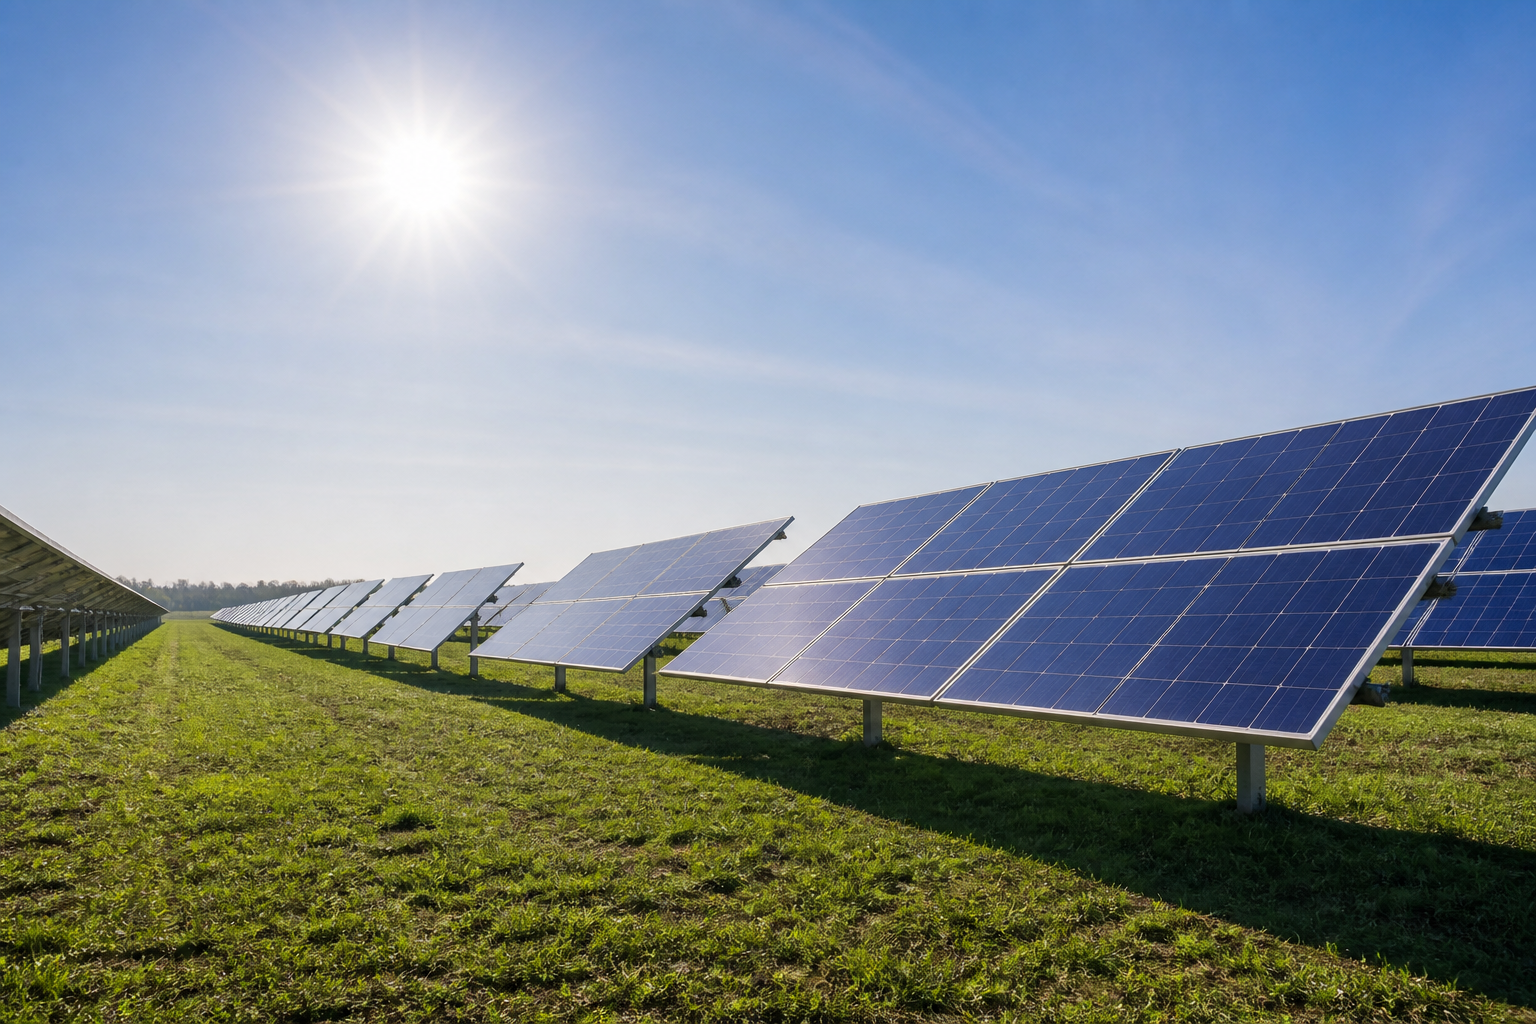
\includegraphics[width=0.58\linewidth]{images/book4/ai/b4-12-solar-farm-sun.png}

{\small Een zonnepark: een kilowatt per vierkante meter poyntingflux komt
vanuit de zon door de lege ruimte aan, en een vijfde daarvan vertrekt door
de kabels.}
\end{omfigure}

\section{Vraagstuk: De energie van een lijn, een paneel en een oven}

\begin{problem}[{Weekendvraagstuk --- de elektromagnetische energie volgen
van een hoogspanningslijn een huis in, van de zon een zonnepaneel in,
en van een magnetron een kop water in}]
\label{pb:b2:poynting-vector:1}

\medskip
\noindent\textbf{Deel I --- De lijn.}
Een coaxiale voedingskabel (kernstraal $a = \qty{1.0}{cm}$, mantelstraal
$b =
\qty{3.0}{cm}$, diëlektricum $\varepsilon_r = 2.3$) voert een
gelijkstroom $I =
\qty{500}{A}$ bij $U = \qty{20}{kV}$; de kern heeft
geleidbaarheid $\gamma =
\qty{6e7}{S/m}$.
\begin{enumerate}
  \item Velden $\vect E(r)$ en $\vect B(r)$ in het diëlektricum (eerst met
        volmaakte geleiders); waarden in $r = a$.
  \item \omterm{thm:b2:poynting-vector:poynting}{Poyntingvector} in het diëlektricum; haar flux door de ringvormige
        doorsnede: ga na dat die gelijk is aan $UI$.
  \item Energiedichtheden $\varepsilon_0\varepsilon_rE^2/2$ en $B^2/2\mu_0$
        in $r = a$ (in een diëlektricum draagt de elektrische
        energiedichtheid $\varepsilon_r$); welke overheerst, en met hoeveel?
  \item Met welke fractie van de lichtsnelheid ``beweegt'' de energie (neem
        $\Pi/u$ in $r = a$)? Vergelijk met $c/\sqrt{\varepsilon_r}$.
  \item De kern biedt nu weerstand: veld $E_z$ erin; de \omterm{thm:b2:poynting-vector:poynting}{poyntingvector} vlak
        buiten haar oppervlak krijgt een radiale component: grootte, en het
        vermogen per meter dat zij aan de kern levert; toets aan $RI^2$ per
        meter.
  \item Verhouding van de radiale tot de axiale component van $\vect\Pi$ in
        $r =
        a$: wat zegt die over waar de energie heen gaat?
  \item Magnetische energie per meter kabel, $\int B^2/2\mu_0\,\dd\tau$, en
        elektrische energie per meter,
        $\int\varepsilon_0\varepsilon_rE^2/2\,\dd\tau$; vind hen terug als
        $\tfrac12\Lambda I^2$ en $\tfrac12\Gamma U^2$ met de zelfinductie en
        de capaciteit per meter uit \cref{ch:b2:dispersion-wave-packets}.
  \item Een lijn van \qty{10}{km}: geleverd vermogen, verloren vermogen,
        fractie. Doe hetzelfde met $U = \qty{200}{kV}$ en $I = \qty{50}{A}$
        (hetzelfde vermogen).
\end{enumerate}

\medskip
\noindent\textbf{Deel II --- Het paneel.}
Zonlicht op het middaguur op een heldere dag: $I = \qty{1.0}{kW/m^2}$; een
fotovoltaïsch paneel van \qty{1.6}{m^2} met een rendement van $20\%$;
fotonenergie gemiddeld \qty{2.0}{eV}.
on average.
\begin{enumerate}[resume]
  \item $E_0$, $B_0$, energiedichtheid en fotonenflux in de bundel.
  \item Geleverd elektrisch vermogen; af te voeren warmte;
        temperatuurstijging als het paneel via beide vlakken warmte verliest
        met $h = \qty{10}{W/(m^2.K)}$.
  \item \omterm{prop:b2:poynting-vector:wave}{Stralingsdruk} op het paneel (absorberend); kracht; vergelijk met
        zijn gewicht (\qty{18}{kg}).
  \item Ontvangen energie per dag (\qty{6}{h} equivalente volle zon) en per
        jaar; oppervlakte die nodig is om een huishouden van
        \qty{3500}{kWh/jaar} te voorzien.
  \item Het paneel levert \qty{30}{V} bij \qty{10.7}{A}: controleer het
        vermogen; poyntingflux langs de \qty{5}{m} tweeaderige kabel naar de
        omvormer --- waar reist dat vermogen, in het beeld van de velden?
  \item Op de baan van de aarde straalt de zon \qty{1.36}{kW/m^2}: totaal
        vermogen van de zon; de massa die zij per seconde omzet ($E = mc^2$,
        $c = \qty{3e8}{m/s}$).
  \item Aantal fotonen dat het paneel per seconde treft.
  \item \omterm{thm:b2:flow-balances:momentum}{Impulsflux} van de fotonen bij de aarde: totale stralingskracht van
        de zon op de aarde (schijf met straal \qty{6400}{km}, absorberend);
        vergelijk met de zwaartekracht (\qty{3.5e22}{N}).
\end{enumerate}

\medskip
\noindent\textbf{Deel III --- De oven.}
Een magnetronoven levert \qty{800}{W} bij \qty{2.45}{GHz} in een holte van
\qty{30}{L}; een kop met \qty{250}{g} water absorbeert daarvan $80\%$.
\begin{enumerate}[resume]
  \item Golflengte; is de holte groot vergeleken daarmee? Waarom zijn de
        wanden van metaal?
  \item Tijd om het water van \qty{20}{\degreeCelsius} tot
        \qty{80}{\degreeCelsius} te verwarmen ($c = \qty{4.18}{kJ/(kg.K)}$);
        geabsorbeerd vermogen per volume-eenheid.
  \item Stroomde het vermogen als een vlakke golf door de doorsnede van
        \qty{50}{cm^2} van de kop, dan: intensiteit en $E_0$; de werkelijke
        velden zijn staande golven met vergelijkbare amplitude --- hoe ver
        liggen de warme plekken uit elkaar, en waarom draait het bord?
  \item Energie die in het veld van de holte is opgeslagen als haar
        kwaliteitsfactor
        $Q = 2\pi\times\text{(opgeslagen energie)}/\text{(energieverlies per periode)}
        \approx 10^3$
        bedraagt wanneer zij leeg is: opgeslagen energie, gemiddelde
        energiedichtheid, $E_0$ --- vergelijk met de doorslag van lucht
        (\qty{3}{MV/m}).
  \item Water absorbeert omdat zijn moleculen dipolen zijn die op
        \qty{2.45}{GHz} worden aangedreven: het lokale joule-achtige
        vermogen is $\tfrac12\omega\varepsilon_0
        \varepsilon''E_0^2$ met
        $\varepsilon'' \approx 10$ voor water: welke $E_0$ in het water is
        nodig voor de vermogensdichtheid van vraag 16; klopt dat?
  \item Fotonenergie bij \qty{2.45}{GHz} in eV, en het aantal fotonen dat de
        kop per seconde absorbeert; waarom microgolven wel kunnen verwarmen
        maar niet ioniseren (ionisatie vraagt zo'n \qty{10}{eV}).
  \item \omterm{prop:b2:poynting-vector:wave}{Stralingsdruk} van het veld in de holte op de wanden (van de orde van
        de energiedichtheid $u$): moet men zich daar zorgen over maken?
  \item Waarom loopt een lege oven (zonder belasting) kans op schade, in
        termen van Poynting?
  \item Vat in een tabel samen, voor de lijn, het paneel en de oven: de
        drager van de energie, de richting van $\vect\Pi$, het vermogen, en
        wat het omzet.
\end{enumerate}
\end{problem}
